\documentclass[12pt,a4paper]{article}

\usepackage[utf8]{inputenc}
\usepackage[T1]{fontenc}
\usepackage{lmodern}
\usepackage[french]{babel}
\usepackage{amsmath,amssymb,amsfonts}
\usepackage{graphicx}
\usepackage{hyperref}
\usepackage{listings}
\usepackage{xcolor}
\usepackage{algorithm}
\usepackage{algpseudocode}

\definecolor{codegreen}{rgb}{0,0.6,0}
\definecolor{codegray}{rgb}{0.5,0.5,0.5}
\definecolor{codepurple}{rgb}{0.58,0,0.82}
\definecolor{backcolour}{rgb}{0.95,0.95,0.92}

\lstdefinestyle{mystyle}{
    backgroundcolor=\color{backcolour},
    commentstyle=\color{codegreen},
    keywordstyle=\color{magenta},
    numberstyle=\tiny\color{codegray},
    stringstyle=\color{codepurple},
    basicstyle=\ttfamily\footnotesize,
    breakatwhitespace=false,
    breaklines=true,
    captionpos=b,
    keepspaces=true,
    numbers=left,
    numbersep=5pt,
    showspaces=false,
    showstringspaces=false,
    showtabs=false,
    tabsize=2
}

\lstset{style=mystyle}

\lstset{
  literate=%
  {é}{{\'e}}1
  {è}{{\`e}}1
  {à}{{\`a}}1
  {ô}{{\^o}}1
  {ç}{{\c{c}}}1
  {É}{{\'E}}1
  {ê}{{\^e}}1
  {î}{{\^i}}1
  {û}{{\^u}}1
  {ë}{{\"e}}1
}

\title{Simulation de Particules en N Dimensions}
\author{Mattéo Audigier \and Mattéo Gautier}
\date{\today}

\begin{document}

\maketitle

\begin{abstract}
Ce rapport présente une implémentation C++ d'un système de simulation de particules en N dimensions. Le projet utilise de nombreuses optimisations pour simuler efficacement les interactions entre particules. Cette bibliothèques ce calcul scientifique permet de modéliser des phénomènes physiques tels que les forces de Lennard-Jones et la gravitation.
\end{abstract}

\vspace{5cm}

\begin{figure}[H]
\centering

\includegraphics[width=0.8\textwidth]{assets/ensimag.png}
\end{figure}

\newpage

\tableofcontents

\newpage

\section{Introduction}

Dans le contexte du développement logiciel, il est important d'avoir des bibliothèques capables de gérer efficacement des simulations, tout en restant rapides, modulaires et simples d'utilisation. Ce projet propose une architecture générique en C++ permettant de simuler des systèmes de particules dans un espace à N dimensions, où N est un paramètre de template. L'objectif est de fournir une base facilement adaptable à divers cas d'usage, et intégrable dans d'autres projets de calcul dynamique de particules.

\subsection{Objectifs du projet}

Les objectifs principaux de ce projet sont:
\begin{itemize}
    \item Concevoir une architecture C++ modulaire et extensible pour la simulation de particules
    \item Disposer d'un projet complet (documentation, tests unitaires, simple à installer), prêt à être repris et étendu par d'autres développeurs
    \item Implémenter un modèle physique incluant forces de Lennard-Jones et gravitation
    \item Optimiser les calculs grâce au partitionnement spatial
    \item Fournir des outils de visualisation via export au format VTK
\end{itemize}

\section{Installation et utilisation}

\subsection{Prérequis}

Pour compiler et utiliser ce projet, il est nécessaire d'avoir:
\begin{itemize}
    \item CMake (version 3.16.3 ou supérieure)
    \item Un compilateur C++ supportant le standard C++17
    \item Doxygen pour la génération de documentation (optionnel)
    \item ParaView pour visualiser les fichiers VTK générés (optionnel)
\end{itemize}

\subsection{Installation}

Pour installer le projet, suivez ces étapes:

\begin{lstlisting}[language=bash]
# Créer un répertoire de build
mkdir build && cd build

# Configurer avec CMake
cmake ..

# Compiler le projet
make
\end{lstlisting}

\subsection{Exécution des tests}

Pour s'assurer que le programme fonctionne correctement, exécutez les tests:

\begin{lstlisting}[language=bash]
make test  # Exécution de tous les tests unitaires
\end{lstlisting}

\subsection{Exécution des démonstrations}

Deux simulations de démonstration sont disponibles:

\begin{lstlisting}[language=bash]
# Simulation de collisions moléculaires
make demo_collision

# Simulation gravitationnelle
make demo_planet

# Afficher l'aide sur les démos disponibles
make demo
\end{lstlisting}

Les fichiers VTK générés dans le répertoire \texttt{demo/nomDeLaDemo} peuvent être visualisés avec ParaView:

\begin{lstlisting}[language=bash]
paraview output_*.vtk
\end{lstlisting}

\subsection{Génération de la documentation}

La documentation API du projet peut être générée grâce à Doxygen:

\begin{lstlisting}[language=bash]
make doc
\end{lstlisting}

La documentation générée est disponible dans le répertoire \texttt{doc/html/index.html}.

\subsection{Optimisations et performance}

Le projet utilise plusieurs niveaux d'optimisations de compilation pour améliorer les performances. Ces options peuvent être modifiées dans le fichier \texttt{CMakeLists.txt} si nécessaire.

\section{Architecture du logiciel}

\subsection{Organisation du projet}

L'arborescence du projet est organisée comme suit:

\begin{verbatim}
root/
|---- CMakeLists.txt          # Configuration CMake principale
|---- Doxyfile.in             # Template pour la documentation Doxygen
|---- README.md               # Documentation principale
|---- include/                # Fichiers d'en-tête (.hpp)
|
|---- src/                    # Implémentations (.cpp, .tpp)
|
|---- demo/                   # Exemples de simulations
|
`---- test/                   # Tests unitaires
\end{verbatim}


Notre simulation est construite autour de cinq classes principales:

\begin{table}[H]
\centering
\begin{tabular}{|c|c|}
\hline
\textbf{Classe} & \textbf{Responsabilité} \\
\hline
Vecteur<N> & Opérations vectorielles en N dimensions \\
\hline
Particle<N> & Propriétés et comportements des particules \\
\hline
Cell<N> & Partitionnement spatial pour optimisation \\
\hline
Univers<N> & Gestion globale de la simulation \\
\hline
VTKconverter<N> & Export des données pour visualisation \\
\hline
\end{tabular}
\caption{Classes principales du système}
\end{table}

\subsection{Diagrammes}

\begin{figure}[H]
\centering
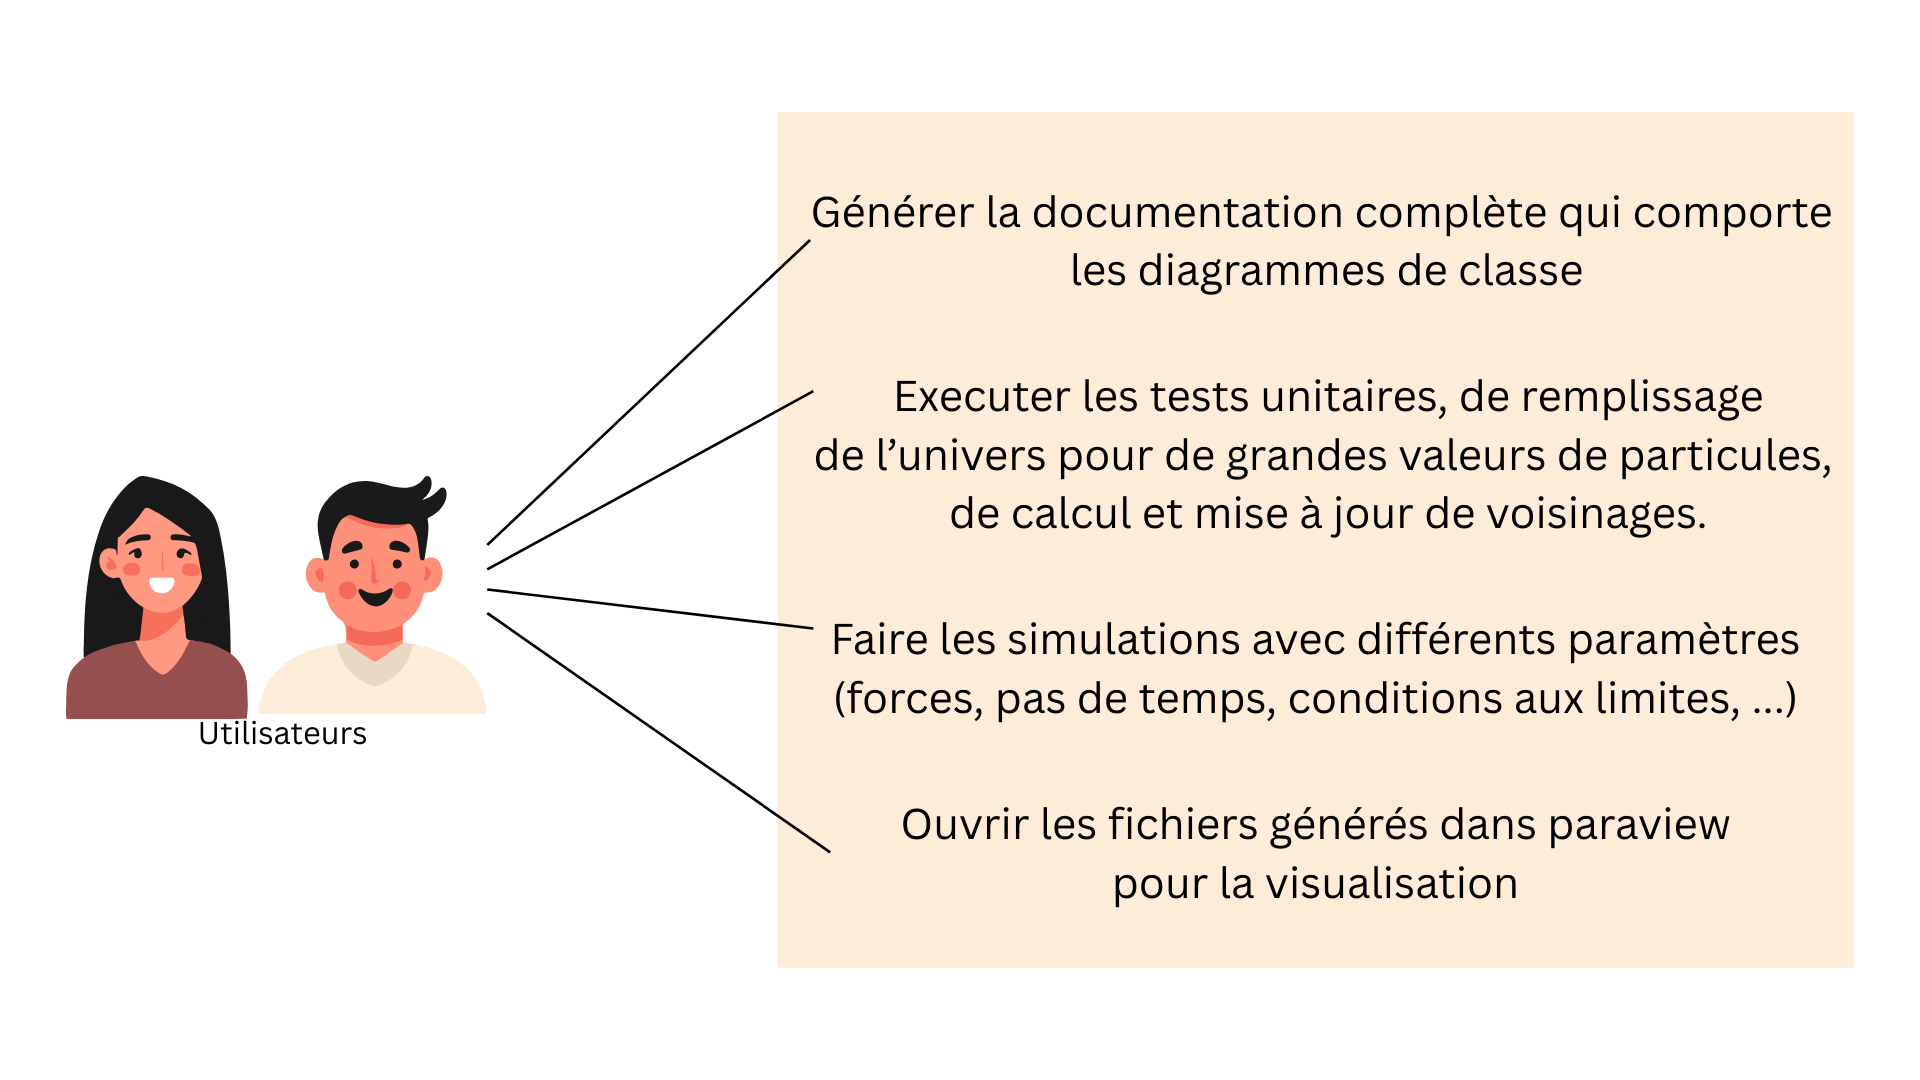
\includegraphics[width=0.8\textwidth]{assets/diagrammeCasUtilisation.png}
\caption{Diagramme de cas d'utilisation}
\end{figure}

\begin{figure}[H]
\centering
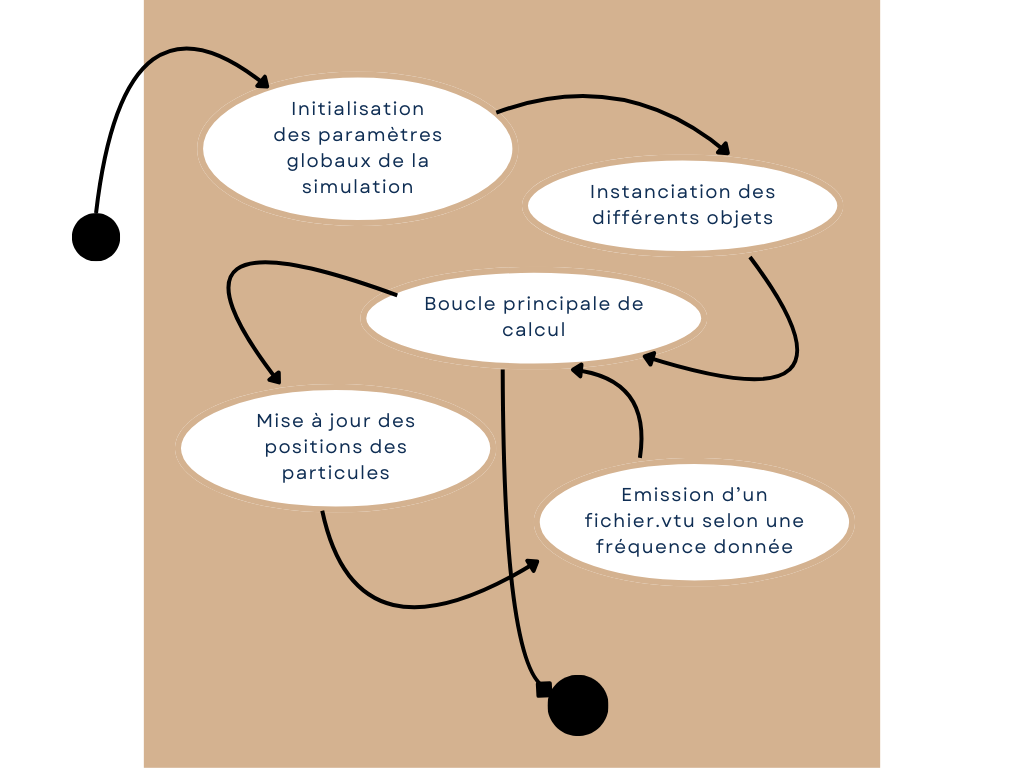
\includegraphics[width=0.8\textwidth]{assets/diagrammeEtatTransition.png}
\caption{Diagramme d'état de la simulation}
\end{figure}

\begin{figure}[H]
\centering
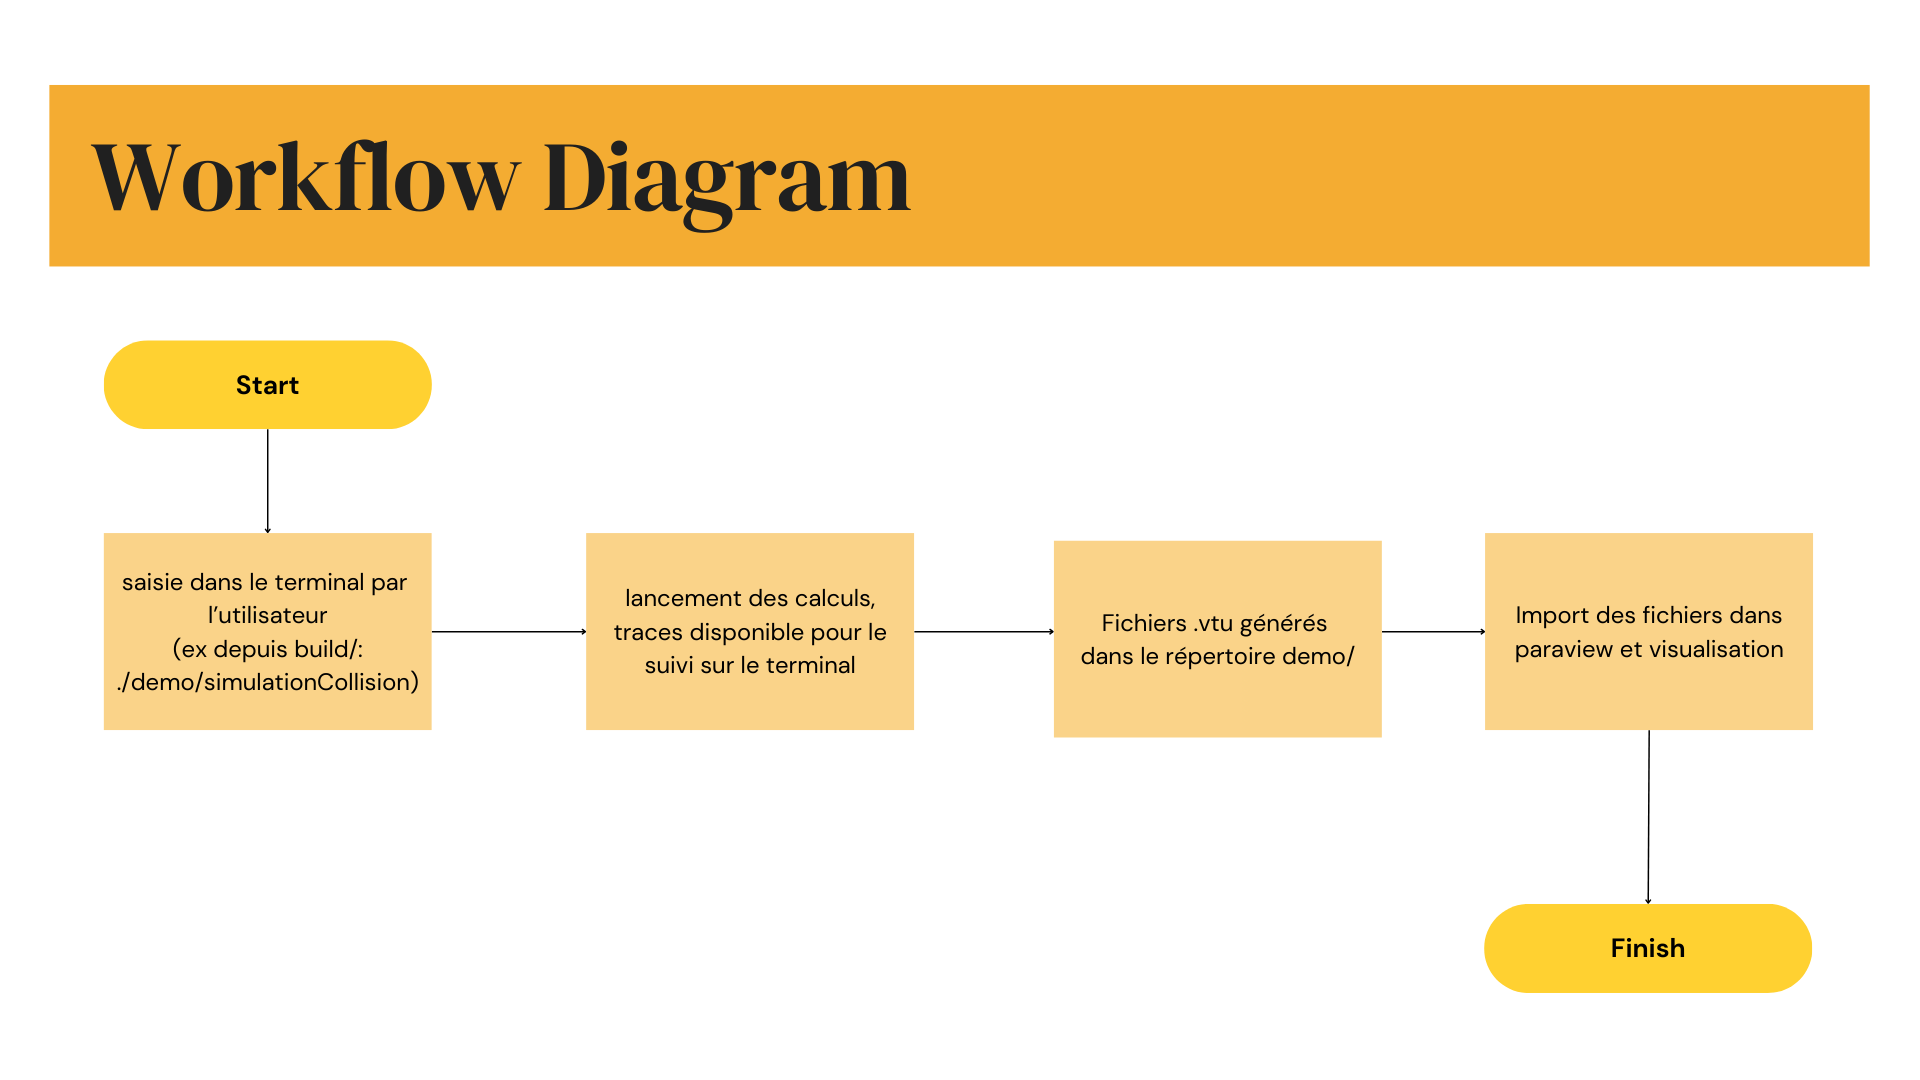
\includegraphics[width=0.8\textwidth]{assets/diagrammeSequence.png}
\caption{Diagramme de séquence de la simulation}
\end{figure}


\subsection{Diagramme UML des classes}

Le diagramme de classes ci-dessous illustre les relations entre les différentes classes du système:

\begin{figure}[H]
\centering
\begin{minipage}{\textwidth}
\begin{verbatim}
+------------+       1..*+-------------+          +--------------+
|   Cell<N>  |-----------| Particle<N> |----------|  Vecteur<N>  |
+------------+           +-------------+          +--------------+
      |1..*
      |
      |
+---------------+1..1    +-----------------+
|   Univers<N>  |--------| VTKconverter<N> |
+---------------+        +-----------------+
\end{verbatim}
\end{minipage}
\caption{Diagramme de classes UML du système}
\end{figure}

\section{Implémentation}

\subsection{Classe Vecteur}

La classe Vecteur représente un vecteur mathématique en N dimensions et implémente toutes les opérations vectorielles nécessaires pour la simulation:

\begin{figure}[H]
\begin{lstlisting}[language=C++, caption=Extrait de la classe Vecteur]
template <std::size_t N>
class Vecteur {
private:
    std::array<double, N> data;

public:
    Vecteur();
    Vecteur(const std::array<double, N>& values);
    double norm() const;
    
    // Operateurs mathematiques
    friend Vecteur<N> operator+(const Vecteur<N>& v1, const Vecteur<N>& v2);
    friend Vecteur<N> operator-(const Vecteur<N>& v1, const Vecteur<N>& v2);
    friend Vecteur<N> operator*(const Vecteur<N>& v, float f);
    friend Vecteur<N> operator/(const Vecteur<N>& v, double d);
};
\end{lstlisting}
\end{figure}

\subsection{Optimisations de la classe Vecteur}

Plusieurs micro-optimisations ont été implémentées dans la classe Vecteur pour maximiser les performances:

\begin{itemize}
    \item \textbf{Allocation statique}: Utilisation de \texttt{std::array} au lieu de \texttt{std::vector} pour un accès plus rapide et une allocation sur la pile
    \item \textbf{Élimination des copies}: Tous les paramètres vectoriels sont passés par référence constante (\texttt{const\&})
    \item \textbf{Optimisations à la compilation}: Utilisation de \texttt{static\_assert} pour vérifier les dimensions à la compilation plutôt qu'à l'exécution
    \item \textbf{Vérification d'auto-affectation}: Test \texttt{if (this != \&other)} dans l'opérateur d'affectation pour éviter un travail inutile
\end{itemize}

\subsection{Classe Particle}

La classe Particle encapsule toutes les propriétés d'une particule et implémente les méthodes pour calculer les forces entre particules:

\begin{figure}[H]
\begin{lstlisting}[language=C++, caption=Extrait de la classe Particle]
template <std::size_t N>
class Particle {
private:
    int id;
    Vecteur<N> position;
    Vecteur<N> velocity;
    double mass;
    std::string category;
    Vecteur<N> force;
    Vecteur<N> old_force;

public:
    // Getters et setters
    int getId() const;
    const Vecteur<N>& getPosition() const;
    
    // Methodes de calcul des forces
    Vecteur<N> optimizedGetAllForces(Particle<N>* p, 
                                     float epsilon_times_24,
                                     float sigma) const;
    
    // Methodes pour le partitionnement spatial
    std::array<int, N> getCellIndexofParticle(double cellLength) const;
};
\end{lstlisting}
\end{figure}

\subsection{Optimisations de la classe Particle}

La classe Particle implémente plusieurs optimisations pour les calculs de forces:

\begin{itemize}
    \item \textbf{Protection contre les forces excessives}: Limitation des forces à des valeurs raisonnables pour éviter les instabilités numériques
    \item \textbf{Précalcul des facteurs constants}: Multiplication préalable d'epsilon par 24 (\texttt{epsilon\_times\_24}) pour éliminer cette multiplication dans chaque calcul
    \item \textbf{Réutilisation des calculs intermédiaires}: Les puissances et distances au carré sont calculées une seule fois puis réutilisées
    \item \textbf{Tolérance numérique}: Utilisation de \texttt{constexpr double alpha = 1e-2} pour éviter les divisions par zéro
\end{itemize}

\subsection{Classe Cell}

La classe Cell implémente le concept de partitionnement spatial pour optimiser les calculs de voisinage:

\begin{figure}[H]
\begin{lstlisting}[language=C++, caption=Extrait de la classe Cell]
template <std::size_t N>
class Cell {
private:
    std::vector<Particle<N>*> particles;
    std::vector<std::array<int, N>> neighbourCellsIndex;
    std::array<int, N> cellIndex;
    double length;
    int numberOfParticles = 0;

public:
    // Construction et gestion des particules
    void addParticle(Particle<N>*& particle);
    void removeParticle(Particle<N>*& particle);
    
    // Acces aux donnees
    std::vector<Particle<N>*> getParticles() const;
    std::vector<std::array<int, N>> getNeighbourCellsIndex() const;
};
\end{lstlisting}
\end{figure}

\subsection{Optimisations de la classe Cell}

La classe Cell optimise le partitionnement spatial:

\begin{itemize}
    \item \textbf{Précalcul des voisins}: Les indices des cellules voisines sont calculés une seule fois puis stockés
    \item \textbf{Test rapide d'appartenance}: Vérification optimisée avec \texttt{isEmpty()} utilisant \texttt{particles.empty()}
\end{itemize}

\subsection{Classe Univers}

La classe Univers est le cœur du système, gérant l'ensemble de la simulation:

\begin{figure}[H]
\begin{lstlisting}[language=C++, caption=Extrait de la classe Univers]
template <std::size_t N>
class Univers {
private:
    std::array<double, N> caracteristicLength;
    double cutOffRadius;
    std::array<int, N> numberOfCells;
    std::unordered_map<std::array<int, N>, Cell<N>*, ArrayHash<N>> cells;
    std::vector<Particle<N>*> particles;
    int nbParticles;

public:
    // Construction et configuration
    Univers(std::array<double, N> caracteristicLength, double cutOffRadius);
    
    // Gestion des particules
    void addParticle(Particle<N>*& particle);
    void updateParticlePositionInCell(Particle<N>* particle, 
                                     const Vecteur<N>& newPosition);
    
    // Calcul des forces et mise a jour
    void computeAllForcesOnParticle(float epsilon, float sigma);
    void update(double dt, float epsilon, float sigma);
    
    // Gestion des conditions limites
    Vecteur<N> applyReflectiveLimitConditions(Particle<N>* particle, 
                                            const Vecteur<N>& newPosition);
};
\end{lstlisting}
\end{figure}

\subsection{Optimisations de la classe Univers}

L'Univers, cœur du système, implémente plusieurs optimisations cruciales:

\begin{itemize}
    \item \textbf{Calcul asymétrique des forces}: Comparaison des IDs (\texttt{particle->getId() < neighbourParticle->getId()}) pour calculer chaque interaction une seule fois, la force étant symétrique
    \item \textbf{Structures de données adaptées}: Utilisation d'une \texttt{unordered\_map} avec une fonction de hachage personnalisée pour accéder rapidement aux cellules
\end{itemize}

\section{Optimisations}

\subsection{Partitionnement spatial}

Le partitionnement spatial divise l'espace de simulation en cellules, permettant de limiter les calculs de forces aux particules voisines. Cette optimisation réduit la complexité des calculs de $O(n^2)$ à $O(n)$ dans des systèmes avec une distribution uniforme de particules.

\subsection{Flags de compilation}

Le projet utilise des flags de compilation avancés pour maximiser les performances. Voici quelques exemples:

\begin{verbatim}
-O3                      # Optimisation de niveau le plus élevé
-march=native            # Optimisations spécifiques à l'architecture
-ffast-math              # Optimisations mathématiques agressives
-funroll-loops           # Optimisation des boucles
-ftree-vectorize         # Vectorisation automatique
\end{verbatim}

\section{Résultats et visualisation}

Les simulations peuvent être visualisées grâce à l'export au format VTK, permettant l'utilisation d'outils comme ParaView pour analyser les résultats.

\subsection{Exemple de simulation}

\begin{figure}[H]
\centering
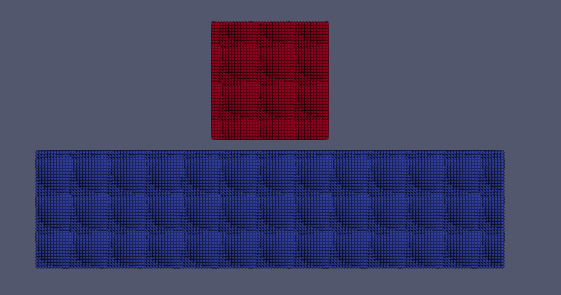
\includegraphics[width=0.8\textwidth]{assets/visu1.png}
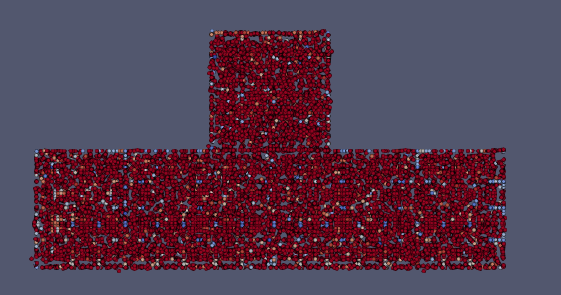
\includegraphics[width=0.8\textwidth]{assets/visu2.png}
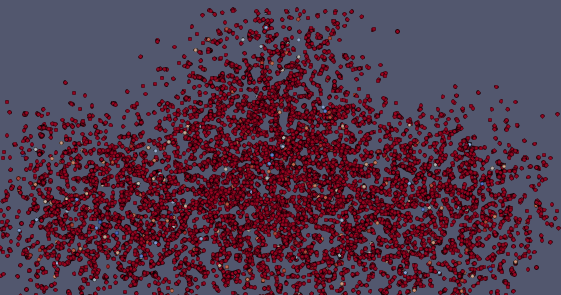
\includegraphics[width=0.8\textwidth]{assets/visu3.png}
\caption{Exemples de visualisation de simulation}
\end{figure}

\section{Performance}

\subsection{Partitionnement spatial}

Le partitionnement spatial permet de réduire le nombre de calculs nécessaires pour déterminer les forces entre particules. En divisant l'espace en cellules, seules les particules dans des cellules voisines sont considérées pour le calcul des forces, ce qui réduit considérablement le temps de calcul.

\begin{figure}[H]
\centering
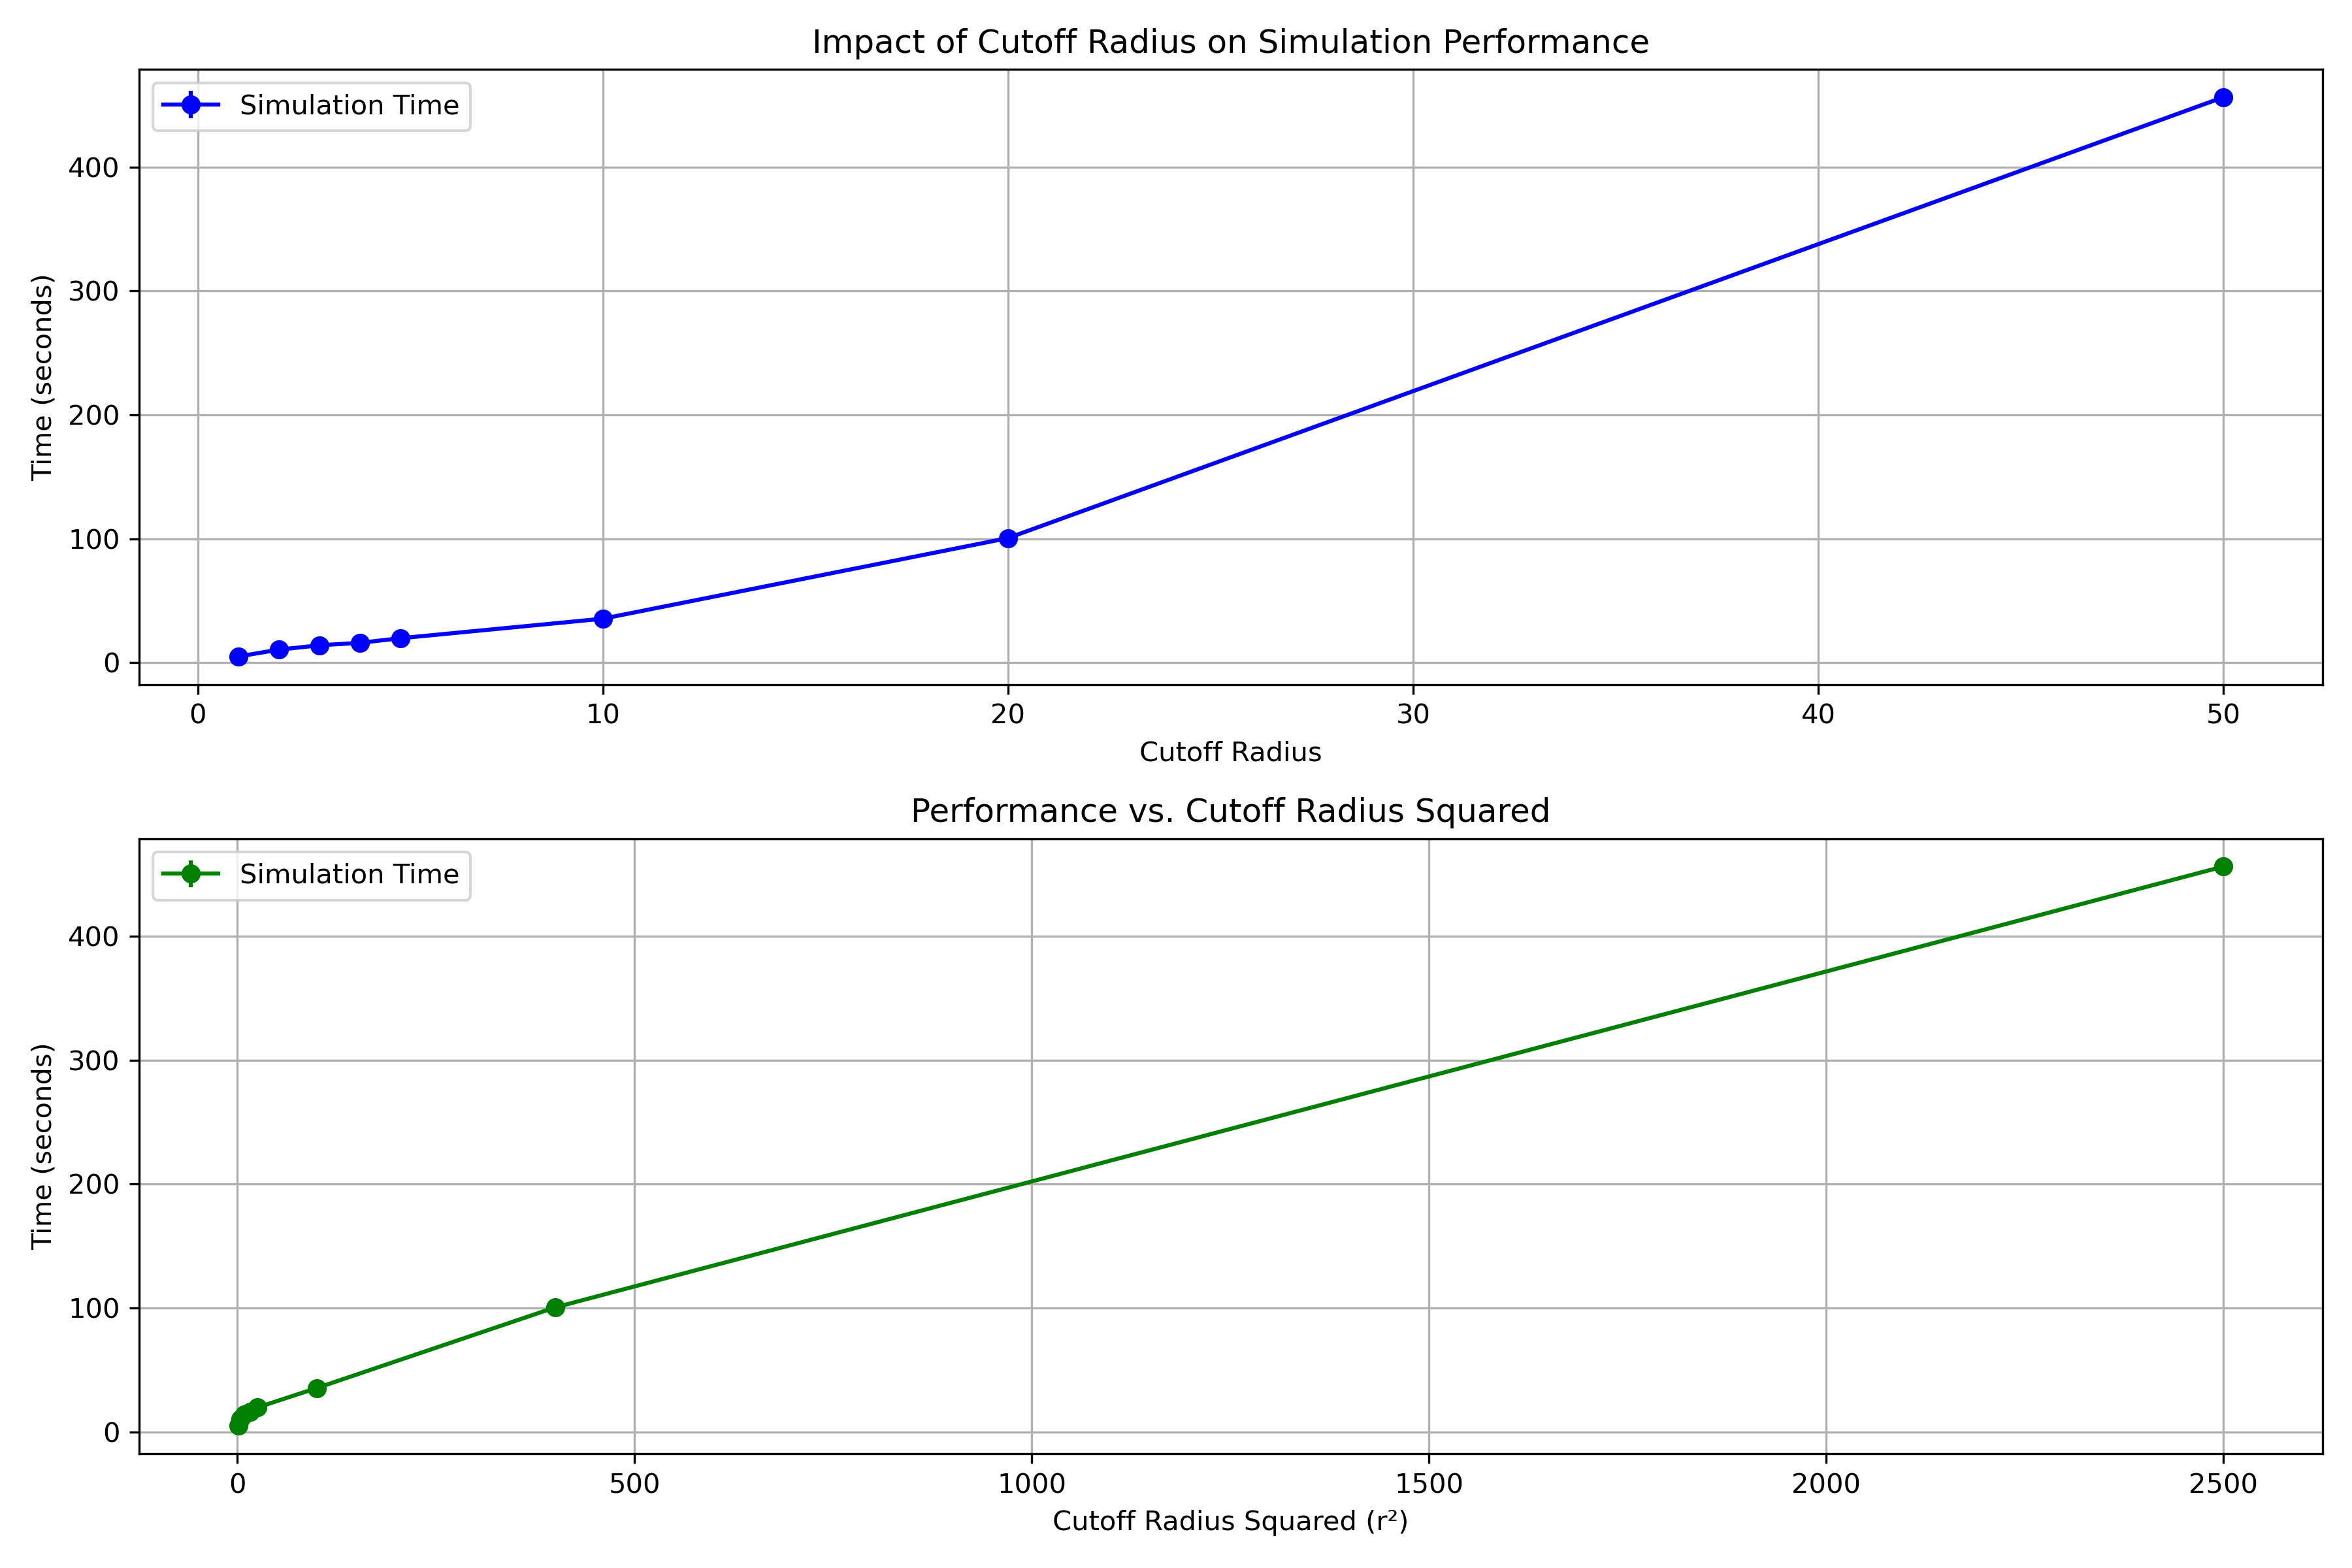
\includegraphics[width=0.8\textwidth]{perf/cutoff_radius_performance.png}
\caption{Temps de simulation en fonction du rayon de coupure}
\end{figure}

\begin{figure}[H]
\centering
\begin{minipage}{\textwidth}
\begin{verbatim}
Performance Summary:
Cutoff     Total Time      Setup Time      Simulation Time
-------------------------------------------------------
1.00       4.95            0.02            4.92           
2.00       10.47           0.00            10.46          
3.00       13.97           0.00            13.97          
4.00       15.97           0.00            15.96          
5.00       19.68           0.00            19.68          
10.00      35.44           0.00            35.44          
20.00      100.51          0.00            100.51         
50.00      456.42          0.00            456.41    
\end{verbatim}
\end{minipage}
\caption{Tableau de performance du partitionnement spatial}
\end{figure}

\subsection{Impact de la génération des VTK}
L'exportation des données au format VTK a un impact sur les performances dû au nombre important d'écriture dans des fichiers nécessaires, mais permet une visualisation efficace des résultats. Le temps d'exportation est proportionnel au nombre de particules et à la complexité de la scène.

\begin{figure}[H]
\centering
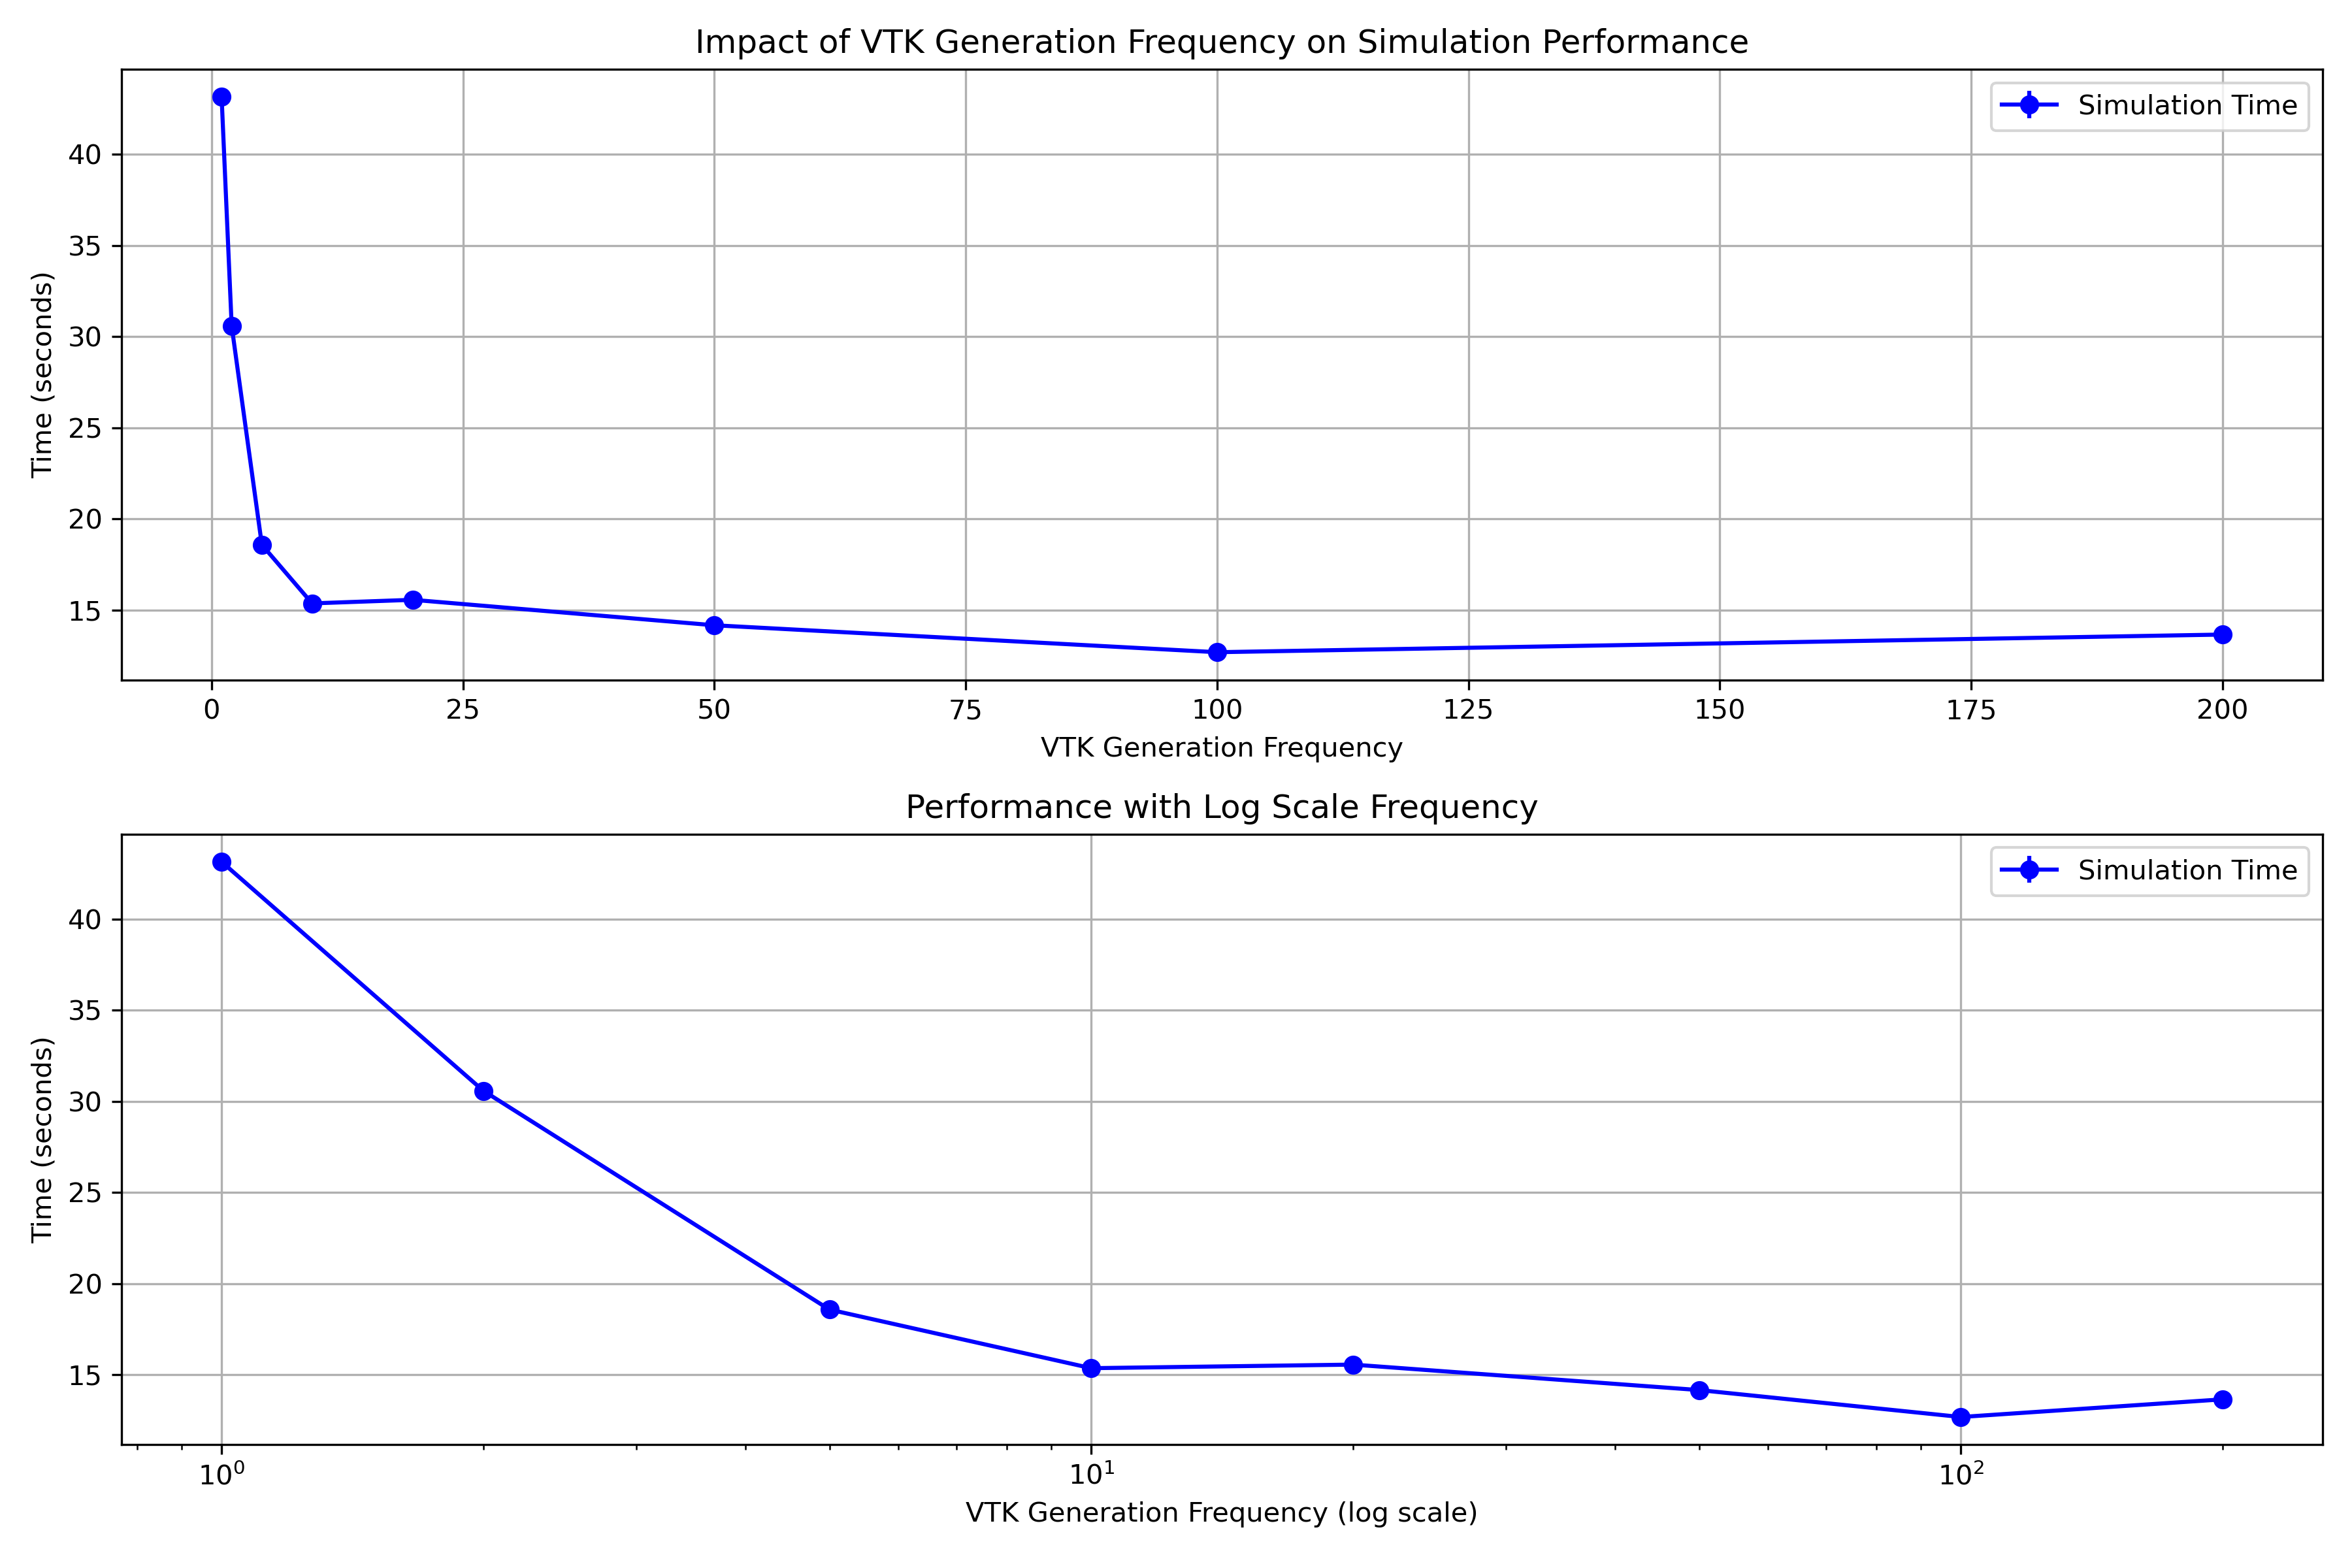
\includegraphics[width=0.8\textwidth]{perf/vtk_frequency_performance.png}
\caption{Temps de simulation en fonction de la fréquence d'exportation VTK}
\end{figure}

\begin{figure}[H]
\centering
\begin{minipage}{\textwidth}
\begin{verbatim}
Performance Summary:
Frequency  Total Time      Setup Time      Simulation Time
-------------------------------------------------------
1          43.15           0.00            43.15          
2          30.59           0.00            30.58          
5          18.59           0.00            18.58          
10         15.37           0.00            15.37          
20         15.57           0.00            15.56          
50         14.17           0.00            14.17          
100        12.69           0.00            12.69          
200        13.66           0.00            13.66    
\end{verbatim}
\end{minipage}
\caption{Tableau de performance de l'exportation VTK}
\end{figure}

\section{Conclusion}

Ce projet démontre l'efficacité d'une approche générique basée sur les templates C++ pour la simulation de particules en N dimensions. L'architecture modulaire et les techniques d'optimisation utilisées permettent de simuler efficacement des systèmes complexes avec un grand nombre de particules.

\subsection{Perspectives}

Plusieurs axes d'amélioration sont envisageables:

\begin{itemize}
    \item L'utilisation du parallélisme pour accélérer les calculs
    \item Ajout de nouveaux modèles physiques (forces électrostatiques, etc.)
\end{itemize}

\end{document}